\documentclass{beamer}
\usepackage{HECbeamer}
\usepackage{icomma}

\title[\color{white}{MATH 60604 \S~5c - Formulation du modèle}]{\texorpdfstring{MATH 60604 \\Modélisation statistique \\ \S~5c - Formulation du modèle}{MATH 60604 \\Modélisation statistique \\ \S~5c - Formulation du modèle}}
\author{Léo Belzile}
\institute{HEC Montréal\\
Département de sciences de la décision}
\date{} 

\begin{document}
\frame{\titlepage}


\begin{frame}[fragile]
\frametitle{Régression linéaire pour les données \texttt{vengeance}}
\bi
\item  Commençons par ajuster un modèle de régression ordinaire, qui nous servira de
point de départ pour la suite. 
\item Ce modèle néglige la possible corrélation intra-personne et fait
comme si les observations étaient indépendantes.
\bi

\item  Le désir de vengeance d'une personne à un temps donné est fort
possiblement corrélé avec celui des autres temps car, justement, il s'agit de la
même personne. 
\item Si c'est le cas, le postulat d'indépendance n'est pas vérifié; il s'ensuit que l'inférence n'est
pas valide.
\ei
\item Le modèle linéaire est
\begin{align*}
\code{vengeance} = \beta_0+\beta_1 \code{sexe} + \beta_2 \code{age} + \beta_3 \code{vc} + \beta_4 \code{wom} + \beta_5 \code{t} + \varepsilon, 
\end{align*}
où les termes d'erreur $\epsilon$ sont supposés indépendants.
\ei
\end{frame}

\begin{frame}[fragile]
\frametitle{Modéliser la progression chronologique}
\bi
\item Il y a deux façons naturelles de modéliser la variable temps:
\bi

\item soit on suppose un effet linéaire entre \code{t} et \code{vengeance} (variable continue).
\item Soit on traite \code{t} comme variable catégorielle. 
\ei

\item  Nous allons utiliser \texttt{proc mixed} pour nous familiariser avec sa syntaxe.
 
\begin{tcolorbox}[olback=white, colframe=hecblue, title=Code SAS pour ajuster un modèle linéaire]
\begin{verbatim}
proc mixed data=modstat.vengeance method=reml;
model vengeance = sexe age vc wom t / solution;
run;
\end{verbatim}
\end{tcolorbox}
\ei
\end{frame}

 \begin{frame}
\frametitle{Sortie du modèle linéaire avec \code{proc mixed}}
\begin{center}
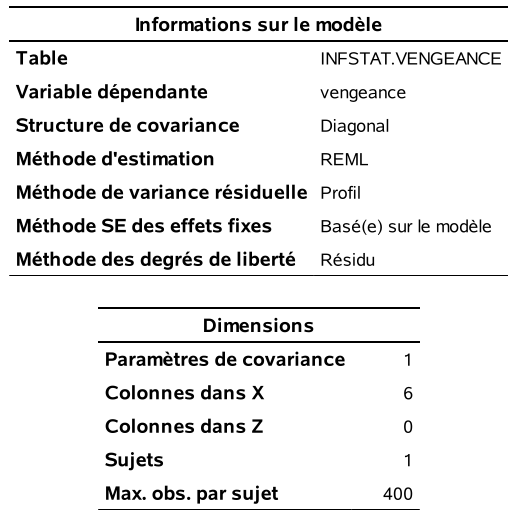
\includegraphics[width = 0.45\linewidth]{img/c5/diapos6-e03}
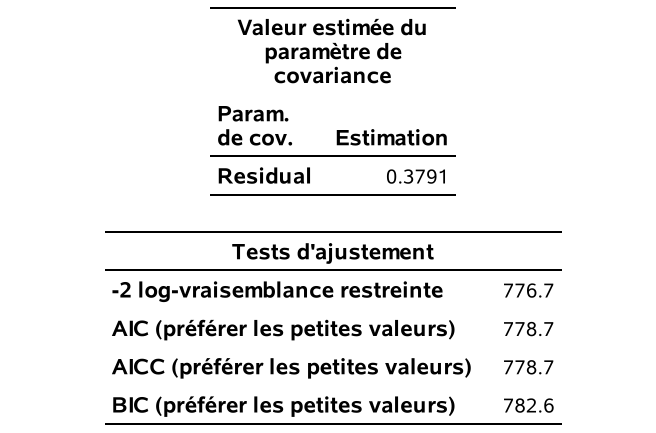
\includegraphics[width = 0.5\linewidth]{img/c5/diapos6-e04}
\end{center}
{\footnotesize La sortie de \code{proc mixed} est plus compliquée que celle de\code{proc glm}.


}

\end{frame}
\begin{frame}
\frametitle{Estimés des coefficients pour la moyenne}
\begin{center}
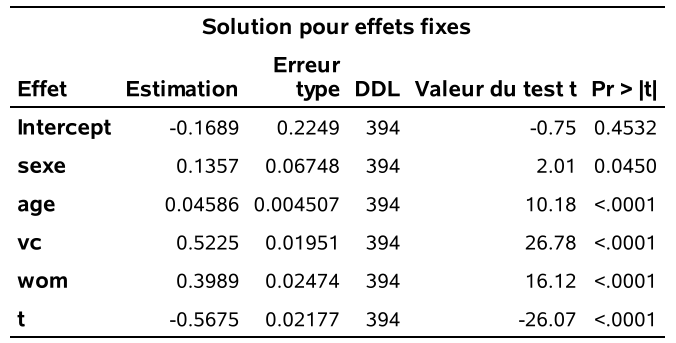
\includegraphics[width = 0.7\linewidth]{img/c5/diapos6-e05}
\end{center}
Les effets de toutes les variables semblent significatifs, quoique tout juste pour \code{sexe}.
\end{frame}

 \begin{frame}
\frametitle{Interprétation des paramètres du modèle linéaire}
\bi
\item  Plus la personne a eu initialement des comportements de type \code{vc} ou \code{wom}, plus le désir de vengeance est élevé. 
\item L'effet du temps est particulièrement d'intérêt ici. On voit qu'il est négatif. À chaque vague successive, la valeur de \code{vengeance} diminue de 0.568, en moyenne, lorsque les autres variables demeurent inchangées. C'est ce qu'on avait vu dans les graphes.
\item \alert{Mais peut-on se fier aux conclusions des tests d'hypothèse?} La réponse est non. L'inférence (tests et intervalles de confiances) est faussée lorsqu'on néglige la dépendance entre les observations.
\ei
\end{frame}


\begin{frame}
\frametitle{Notations}
\bi
\item Supposons qu'on dispose de $m$ groupes d'observations tels que:
\be
\item Il y a $n_i$ observations dans le groupe $i$ ($i=1, \ldots, m$).
\item Deux observations d'un même groupe sont possiblement corrélées.
\item Deux observations provenant de deux groupes distincts sont
indépendantes.
\ee
\item Les groupes peuvent être formés de plusieurs manières:
\bi
\item Plusieurs mesures peuvent être prises sur un même sujet (mesures répétées) et chaque individu forme alors un groupe. 
\item Un groupe peut aussi être formé
d'individus d'une même école, d'une même unité ou département au travail ou
d'une même famille. 
\ei
\item Comme par le passé, nous allons supposer que nous avons une variable réponse
 et un ensemble de $p$ variables explicatives.
\item Pour simplifier la notation, on dénote par $\mathbf{X}_i$ l'ensemble des variables aléatoires pour le groupe $i$.
\ei
\end{frame}


\begin{frame}
\frametitle{Notations}
\bi
\item On utilise l'indice $i$ pour indiquer le groupe et $j$ pour indiquer la $j$e observation au sein du groupe $i$.
\bi

\item Si le groupe est une entreprise, $i$ dénote l'entreprise, et $j$ dénote le sujet.
\item Pour des données longitudinales, $i$ représente le sujet et $j$ la mesure à un \textbf{temps} donné.
\ei
\item On note $\bs{Y}_i=(Y_{i1}, \ldots, Y_{in_i})$ l'\alert{ensemble des observations} de la variable d'intérêt pour le groupe $i$. 
\item Pour les variables explicatives, on a maintenant besoin de trois indices:
\bi \item $i$ pour le groupe
\item $j$ pour le numéro d'observation au sein du groupe
\item  $k$ pour la variable explicative.
\ei
\item On note donc  $\mathbf{X}_{ij}=(1, \mathrm{X}_{ij1}, \ldots, \mathrm{X}_{ijp})$ l'ensemble des $p$ variables explicatives pour l'observation $j$ du groupe $i$.
\ei
\end{frame}

\begin{frame}
\frametitle{Modèle linéaire avec corrélation sur les erreurs}
 Le modèle de régression linéaire peut s'écrire
\begin{align*}
Y_{ij}=\beta_0+\beta_1\mathrm{X}_{ij1}+\cdots+\beta_p \mathrm{X}_{ijp}+\varepsilon_{ij}
\end{align*}
pour $i=1, \ldots, m$ et $j=1, \ldots, n_i$, où $\varepsilon_{ij}$ est le terme d'erreur de l'observation $j$ du groupe $i$.
\bi
\item Comme avant, on suppose que $\E{\varepsilon_{ij}\mid  \mathbf{X}_{ij}}=0$ et donc 
\begin{align*}
\E{Y_{ij}\mid \mathbf{X}_i}=\beta_0+\beta_1\mathrm{X}_{ij1}+\cdots+\beta_p \mathrm{X}_{ijp}. \end{align*}
% 
% \item Par contre, \alert{on ne suppose plus que les erreurs sont indépendantes}.
\ei
\end{frame}
\begin{frame}
\frametitle{Structure de covariance/corrélation}
\bi
\item Puisqu'on assume les variables explicatives $\mathbf{X}$ fixes dans le modèle, parler de structure de corrélation des erreurs $\bs{\varepsilon}$ est équivalent à parler de la structure de corrélation des observations $\bs{Y}$.
\item Nous allons permettre la
dépendance entre les observations d'un même groupe. 
\item On suppose les groupes indépendants, donc $\Co{\eps_{ij}, \eps_{i'j'}}=0$ si $i \neq i'$.
\item On modélise la corrélation  \alert{intra-groupe} en assumant que la matrice de covariance des $\bs{Y}$ du groupe $i$ est
\begin{align*}
\Co{\bs{Y}_i\mid \mathbf{X}_i}=\bs{\Sigma}_i, 
\shortintertext{
ou, de manière équivalente, }
\Co{\bs{\varepsilon}_i\mid \mathbf{X}_i}=\bs{\Sigma}_i, 
\end{align*}
où $\bs{\varepsilon}_i=(\varepsilon_{i1}, \ldots, \varepsilon_{in_i})$ est le vecteur des erreurs du groupe $i$.
\ei
\end{frame}


\begin{frame}
\frametitle{Covariance par blocs pour données longitudinales}
\bi 
 \item 
 Supposons sans perte de généralité que les données sont ordonnées par groupe. 
 \item On suppose que les observations d'un groupe $i$ sont corrélées, mais que les observations de groupes différents sont indépendantes.

 \item Alors, la matrice de covariance de toutes les  \textbf{observations} est \textbf{diagonale par blocs}:
 \begin{align*}
  \Co{\bs{Y}} = \begin{pmatrix}
                 \bs{\Sigma}_1 & \mathbf{O} & \cdots & \mathbf{O}\\
                  \mathbf{O} &\bs{\Sigma}_2 & \cdots & \mathbf{O} \\
                  \vdots & \ddots & \ddots & \vdots \\
                   \mathbf{O} & \mathbf{O} & \cdots & \bs{\Sigma}_m 
                \end{pmatrix}.
\end{align*}
\bi 
\item Dans notre exemple \texttt{vengeance}, on a $n=80 \times 5 = 400$ observations.
\item La matrice de covariance \alert{intra-groupe}, $\bs{\Sigma}_i$, est $5 \times 5$ parce que notre échantillon équilibré ($n_1 = \cdots = n_m=5$). Le bloc $\bs{\Sigma}_i$ est identique peu importe le groupe.
\item La covariance \textbf{inter-groupe} est \textbf{nulle} ($\mathbf{O}$) parce qu'on suppose que les données d'individus différents sont indépendantes les unes des autres.
\ei
\ei
\end{frame}



\begin{frame}
\frametitle{Structure de covariance/corrélation}
\bi
\item En général, la structure de covariance dépendra de quelques paramètres qui
seront estimés au même titre que les paramètres $\bs{\beta}$. 
\item La structure de
covariance sera habituellement spécifiée par l'analyste. Il n'est pas rare qu'il
faille essayer plus d'une structure de covariance pour déterminer celle qui
convient le mieux aux données. 
\item Nous reviendrons sur le problème du choix de
la structure de covariance plus tard, mais nous présentons dès maintenant une
structure de covariance, parmi les plus simples. 
\ei
\end{frame}
\end{document}
